\documentclass{beamer}
\usepackage[UTF8]{ctex}
\usepackage{graphicx}

\title{C语言程序设计安全项目}

% \subtitle{}

\author{李梓勤}

\institute{四川大学网络空间安全学院}

\begin{document}
\begin{frame}
    \titlepage
\end{frame}
\begin{frame}{Intros}
    此报告主要基于我发布在我博客上的三篇文章,\href{https://tiger1218.com/2022/12/19/scuccs-c-security-lab1/}{Decoding Lab}, \href{https://tiger1218.com/2022/12/20/scuccs-c-security-lab2/}{bufbomb}和\href{https://tiger1218.com/2022/12/21/scuccs-c-security-lab3/}{Bomb Lab}。
    
    在解题过程中需要用到的所有文件都已被存储在\href{}{我的Github仓库}中。每个Lab的每个Section的编译选项都已注明。
\end{frame}
\begin{frame}{Lab1}{Key1 \& Key2}
    根据 \texttt{guide.html},我们首先只需要考虑 \texttt{key1}和 \texttt{key2};而我们应该要得到一串解密后的字符串,以 \texttt{From:}开头。审计函数 \texttt{extract\_message1},经过黑盒 \& 白盒测试,我们可以发现该函数会从 \texttt{start+1}处开始,每 \texttt{stride}个字符,drop一个字符。
    
    定位 \texttt{F,r,o,m}。最后得出 \texttt{start=9 \& stride=3}。\texttt{start}为dummy(在内存中)的第一个byte,  \texttt{stride}为dummy(在内存中)的第二个byte。

    然而Linux和Windows都是小端序,所以正确的解释是: \texttt{start}是dummy的Least Significant Byte, \texttt{stride}则是次低位。

    也就是 \texttt{dummy}应该为0x????0309。?可以取任何值。

    看到 \texttt{process\_keys12},该函数可以视为一个任意内存写:将 \texttt{key1}赋值为 \texttt{\&key1}相对于指定修改内存的偏移, \texttt{key2}为指定修改的值。一种可能的解法就是修改 \texttt{dummy}。我们可以用反汇编软件或gdb知道 \texttt{\&dummy}与 \texttt{\&key1}的偏移。
\end{frame}
\begin{frame}{Lab1}{Key3 \& Key4}
    观察得知:

    \begin{enumerate}
        \item 与 \texttt{process\_keys12}一样, \texttt{process\_keys34}也是一个任意内存写。
        \item 除非修改了 \texttt{data}、 \texttt{start}或者 \texttt{stride}, \texttt{extract\_message1}执行后一定会使得 \texttt{msg1}不等于空。
        \item  \texttt{start}和 \texttt{stride}应该不变;不然 \texttt{extract\_message2}的返回值, \texttt{msg2}就会被修改
        \item  \texttt{process\_keys34}会执行两次; \texttt{process\_keys34}的修改又是偏移性质,所以两次对内存的修改结果可能不一样。
    \end{enumerate}
\end{frame}

\begin{frame}{Lab1}{Key3 \& Key4}
    在这里仅简述第一种做法。

    一个 \texttt{int}是4个bytes,所以key3应该为4,才能修改栈上的返回值。

    $ \mathrm{0x14f7}-\mathrm{0x14c6}=49 $

    因此key4就是49。

    所以第二阶段的payload为 \texttt{./lab1 -1 0x0309 4 49}。
\end{frame}

\begin{frame}{Lab2}{Solution1}
    这道题的最低利用条件应该是  \texttt{No Canary}+ \texttt{No PIE}。

    审计题目源码后最容易发现的解法应该是跳过赋值语句,直接到 \texttt{printf}语句。

    如以上代码所述,在 \texttt{0x80492d2}处执行完 \texttt{getbuf},接下来是把返回值(即 \texttt{eax})压进栈中,然后再把字符串(即 \texttt{getbuf returned \%x\\n})地址压入栈中。因为我们可以通过 \texttt{getxs}操作整个 \texttt{getbuf}函数的栈,又因为 \texttt{test}函数调用了 \texttt{getbuf}函数————也就是 \texttt{test}在 \texttt{getbuf}逻辑意义上的上面(或者物理意义的下面),我们也可以操纵整个 \texttt{test}的栈。这样第一种利用 \texttt{printf}语句的方法就很容易得出了:跳到 \texttt{0x80492e0},然后控制栈顶使栈顶为0xdeadbeef。
\end{frame}

\begin{frame}{Lab2}{Solution1}
    显然栈抬升了0x18个Bytes(注意栈从高向低生长)。因此我们的Payload需要加上0x18个Bytes的填充。

    程序为32位程序;那么Payload还需要加上0x04个Bytes来填充edp。

    最后我们需要将存储的eip指针覆盖为我们想要去的地址,也就是 \texttt{0x80492e0},并且使得覆盖完后的栈顶\footnote{基本的\href{https://www.cnblogs.com/clover-toeic/p/3755401.html}{C语言函数调用栈}知识可以看这篇文章。}为0xdeadbeef。(注意Linux x64是小端序机器)

    这是一种Payload:00000000 00000000 00000000 00000000 00000000 00000000 00000000 E0920408 EFBEADDE
\end{frame}

\begin{frame}{Lab2}{Solution2}
    另外一个非常容易想到的思路和 \texttt{ret2libc}\footnote{在CTF-Wiki上简述了\href{https://ctf-wiki.org/pwn/linux/user-mode/stackoverflow/x86/basic-rop/\#ret2libc}{ret2libc}的原理和利用方法。}非常像。

    我们完全可以不使用 \texttt{0x080492e7}处的 \texttt{printf}————我们可以自己构造一个出来!

    字符串的地址是 \texttt{0x0804A019},第二个参数应为0xdeadbeef,所以根据i386架构下的 \texttt{ret2libc}原理,我们可以写出以下payload:

    padding + ebp + (target address) + (return address) + arg1 + arg2 + arg3 ... 
\end{frame}

\begin{frame}{Lab2}{Solution2}
    与solution1中一样,padding为0x18Bytes,ebp为0x04Bytes。目标函数为 \texttt{printf}在plt表中的位置。return function可以不填。arg1为 \texttt{0x0804A019},arg2为0xdeadbeef。

    从上至下依次是28Bytes的padding zeros,目标函数地址,返回地址,参数1,参数2。

    payload: ``00000000 00000000 00000000 00000000 00000000 00000000 00000000 50900408 00000000 19A00408 EFBEADDE''
\end{frame}

\begin{frame}{Lab3}{Solution3}
    接下来我们来讨论在关闭 \texttt{NX}保护和关闭 \texttt{ASLR}保护的利用情况。\footnote{\href{https://stackoverflow.com/questions/2340259/how-to-turn-off-gcc-compiler-optimization-to-enable-buffer-overflow}{How to turn off gcc compiler optimization to enable buffer overflow? - stackoverflow}}

    我们可以回顾一下程序的各个section基本情况:

    \begin{enumerate}
        \item .code段有读、执行权限,但是没有写权限
        \item .data、heap、通常情况下的stack段,都是只有读写权限
        \item .rodata只有读权限
    \end{enumerate}
\end{frame}

\begin{frame}{Lab3}{Solution3}
    一般来说,写权限和执行权限应该尽量分开。这种保护方法就叫NX保护————或者No eXecute保护。

    但是如果我们主动在gcc编译中关闭NX保护,那我们就可以得到一个RWX段,也就是同时有读、写、执行权限的段,栈。

    这时我们可以考虑将shellcode写在栈上,然后劫持控制流到shellcode的开始处。这时Payload应具有下面的结构:

    shellcode + padding + ebp + shellcode's start addr
\end{frame}

\begin{frame}{Lab3}{Solution3}
    第二个问题出现了。shellcode写在栈上,虽然我们可以通过关闭NX保护将shellcode从不可执行变成可执行,但是我们并不知道shellcode的地址。每次我们运行程序的时候,内核都会随机加载程序的地址空间。

    Problem solved!

    当跳转到0x80492d7后,这一切就像无事发生,只不过返回值,也就是 \texttt{eax}会被改成0xdeadbeef。\footnote{我们可以使用\href{https://docs.pwntools.com/en/stable/asm.html}{PWNTools中的ASM模块}来将汇编代码编译成字节码。}

    跳转到0x80492e0也就意味着跳过了push第二个参数。因此,我们可以直接通过栈操作到给第二个参数赋值。

    当然,既然我们可以执行任意汇编代码了,那我们有很多种方法来使得输出达到我们想要的结果。
\end{frame}

\begin{frame}{Lab3}{Solution4}
    既然我们可以执行任意汇编代码,那我们为什么不试着拿Shell权限呢?首先我们需要找到一个放置Shellcode的地方。

    回到我们前面给到的这个结构: shellcode + padding + ebp + shellcode's start addr 

    \texttt{padding + ebp}一共是24Bytes,但是考虑到Shellcode执行阶段可能遇到的 \texttt{push}指令,更好的选择其实是放在 \texttt{shellcode's start addr}的后面。

    这时我们的payload就变成了下面的结构:

    padding + ebp + shellcode's start addr + shellcode
\end{frame}

\begin{frame}{Lab2}{Solution4}
    在网上找一个小一点的Shellcode\footnote{利用int 0x80执行了/bin/sh的一段\href{https://shell-storm.org/shellcode/files/shellcode-841.html}{Shellcode}},我们就得到了我们最终的Payload:

    00000000 00000000 00000000 00000000 00000000 00000000 EBP START\_ADDR 31C9F7E1 B00B5168 2F2F7368 682F6269 6E89E3CD 80
\end{frame}

\begin{frame}{Lab2}{Solution4}
    \begin{figure}[h]
        \centering
        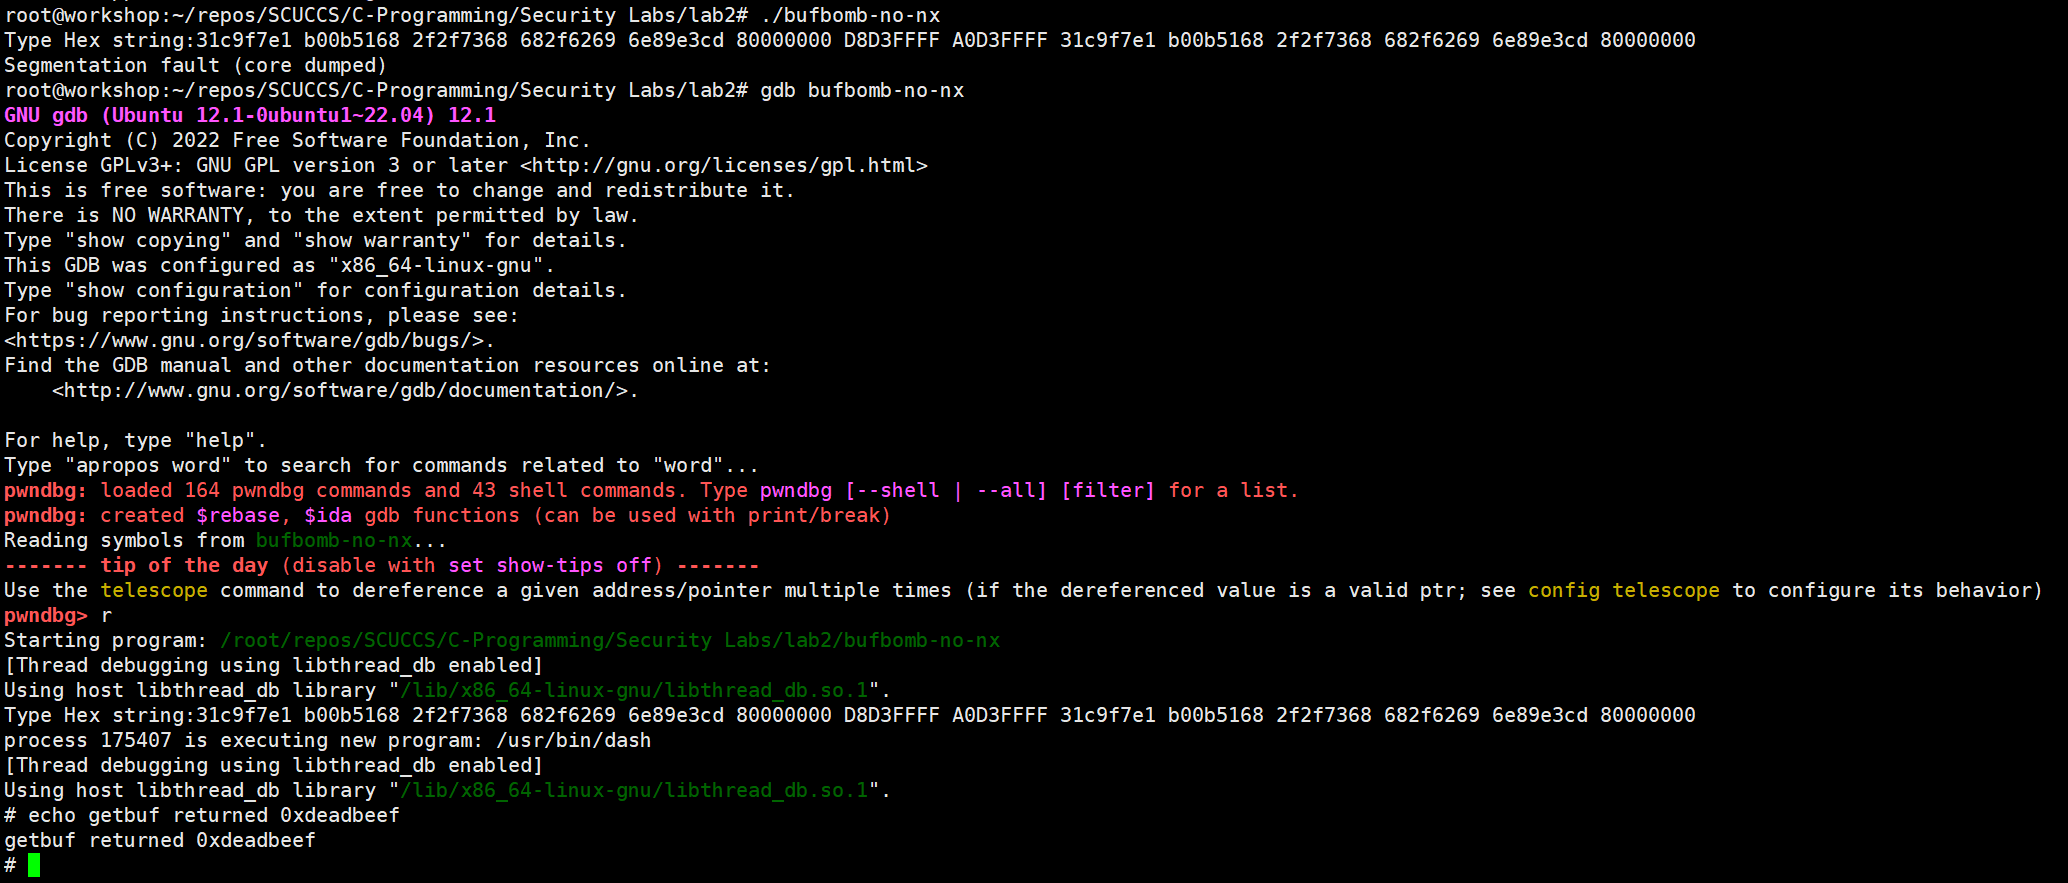
\includegraphics[width=1\textwidth]{images/final_sh_shellcode}
        \caption{彩蛋:拿到shell后直接输出`getbuf returned 0xdeadbeef'}
    \end{figure}
\end{frame}

\begin{frame}
    \centering \Large
    \emph{Thank you!}
\end{frame}

\end{document}